Nachtrag zu Eintrag 5:
Die Analogie zum ohm'schen Gesetz aus der Elektronik bezogen auf die Wärmelehre hilft ungemein beim Verständnis.
Insbesondere durch Lösen der Aufgabe 6 auf Folie 94 und die damit einhergehende Erkenntnis wie sich die
Zusammenhänge easy auf andere Situationen übertragen lassen ist gewissermaßen augenöffnend.

\begin{figure}[h]
    \centering
    \subfloat[Analogie aus der ET]{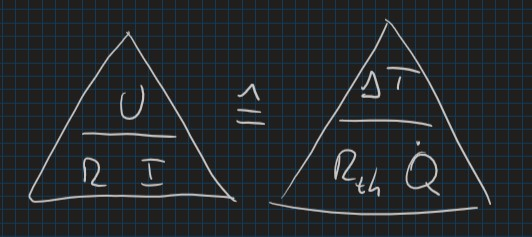
\includegraphics[width=0.4\linewidth]{entries/6/uri.jpg}}
    \qquad
    \subfloat[Grundgleichung Wärmestrom]{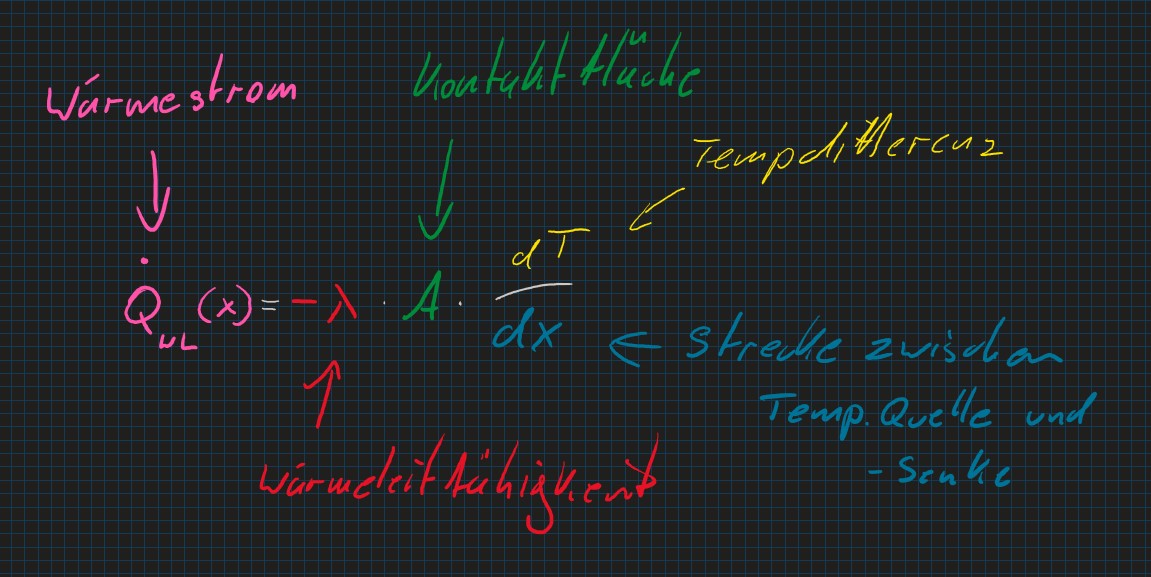
\includegraphics[width=0.4\linewidth]{entries/6/waermestrom.jpg}}
    \caption{Wärmeleitung und URI bzw. \(\Delta T R_{th} \dot{Q}\)}
    \label{fig:strom}
\end{figure}

Ohne die gesamte Aufgabe zu rezitieren war in Aufgabenteil \textbf{b)} gefragt welche Wassertemperatur sich im Inneren
der Leitung bei gegebener Außentemperatur einstellen würde. Mit der Überlegung, dass der Wärmestrom ausschließlich in
radialer Richtung stattfindet gibt mir die Gleichung aus \bild{fig:strom} etwas umsortiert

\begin{equation}
    \frac{- \dot Q}{\lambda} \cdot \int_{}^{} \mathrm{d}A = \int_{T_1}^{T_2} \mathrm{d}T = T_2 - T_1 = \Delta T
    \label{eq:1}
\end{equation}

Die Wasserleitung folgt zylindrischer Geometrie. Betrachtet wird bloß ein Streckenabschnitt von einem Meter (da die
Heizleistung ebenfalls auf einen Meter Länge bezogen ist). Somit ist das (im Kontext der Aufgabenstellung)
Flächenelement \(dA\) nur noch abhängig vom Radius und das Integral aus \gl{eq:1} vereinfacht sich zu

\begin{gather}
    \Delta T = \frac{- \dot Q}{2 \pi l \lambda} \cdot \int_{r_1}^{r_2} \frac{1}{r} \mathrm{d}r = \frac{- \dot Q}{2 \pi l \lambda} \cdot \ln \left(\frac{r_2}{r_1}\right) \nonumber\\
    \Delta T = - \dot{Q} \cdot R_{th}\\
    \text{mit} \nonumber\\
    R_{th} = \frac{1}{2 \pi l \lambda} \cdot \ln \left(\frac{r_2}{r_1}\right)
    \label{eq:2}
\end{gather}

Da die Heizleistung \(P = \SI{8}{W}\) gerade gleich dem Wärmestrom \(\dot{Q}\) ist und der Aufbau der Rohrleitung einer
Reihenschaltung von Widerständen mit geometrisch identischen Charakteristika entspricht ergibt sich die
Temperaturdifferenz \(\Delta T\) zwischen Wasser und Außenluft zu

\begin{gather}
    \Delta T = - P \cdot \sum_{i} \frac{1}{2 \pi l \lambda_i} \cdot \ln \left(\frac{r_{2,i}}{r_{1,i}}\right)
\end{gather}

Welche Augen öffnets? Ich kann plötzlich hiermit etwas anfangen

\begin{figure}[h]
    \centering
    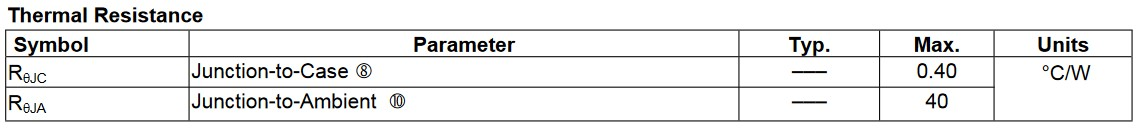
\includegraphics[width=\textwidth]{entries/6/irfs7530.jpg}
    \caption{Ausschnitt aus dem Datenblatt des \textcolor{blue}{\href{https://www.infineon.com/dgdl/irfs7530-7ppbf.pdf?fileId=5546d462533600a40153563a9d1e21d8}{IRFS7530}} von Infineon}
    \label{fig:thermalResi}
\end{figure}
\vspace{40mm}
\begin{figure}[h]
    \centering
    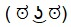
\includegraphics[width=0.07\textwidth]{entries/6/ha.jpg}
\end{figure}
\newpage
\textbf{Weiter}

Das Kirchhoff'sche Strahlungsgesetz (ja, der gleiche Edelmann der nach ihm benannten Regel aus der elektrotechnik) besagt,
dass ein Körper ebenso viel Leistung abstrahlt wie absorbiert wurde oder mit anderen Worten - ein realer Körper ist ein
ebenso guter Strahler wie absorber. Die abgestrahlten Wellenlängen müssen hierbei nicht den absorbierten entsprechen!
\begin{figure}[h]
    \centering
    \subfloat[Intensitätsverteilung absorbierter Wellenlängen. Gepunktet: tatsächlich eingestrahlte Intensität, Durchgezogen: absorbierte Anteile]{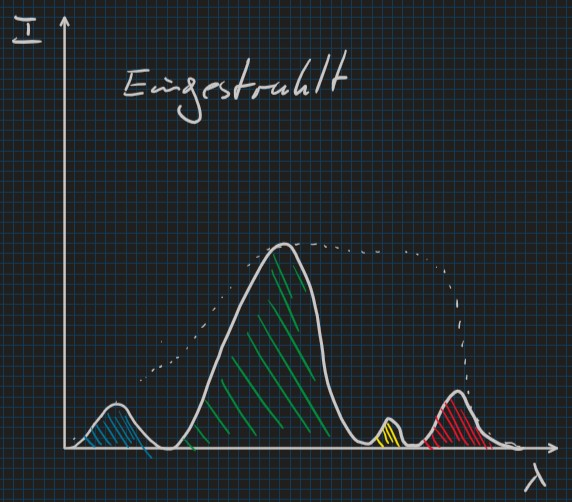
\includegraphics[width=0.4\linewidth]{entries/6/eingestrahlt.jpg}}
    \qquad
    \subfloat[Intensitätsverteilung emittierter Wellenlängen.]{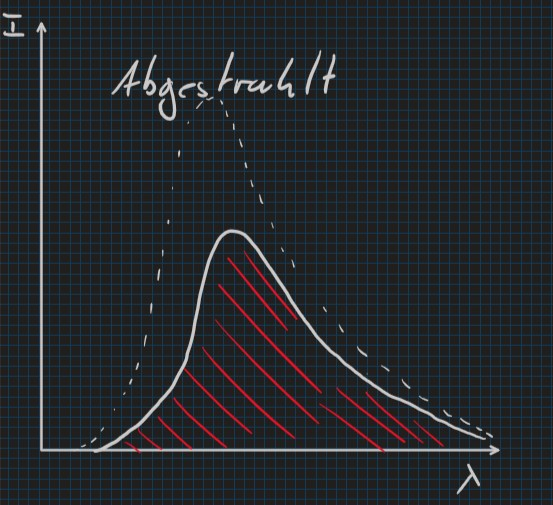
\includegraphics[width=0.4\linewidth]{entries/6/abgestrahlt.jpg}}
    \qquad
    \subfloat[Intensitätsverteilung absorbierter Wellenlängen des schwarzen Körpers.]{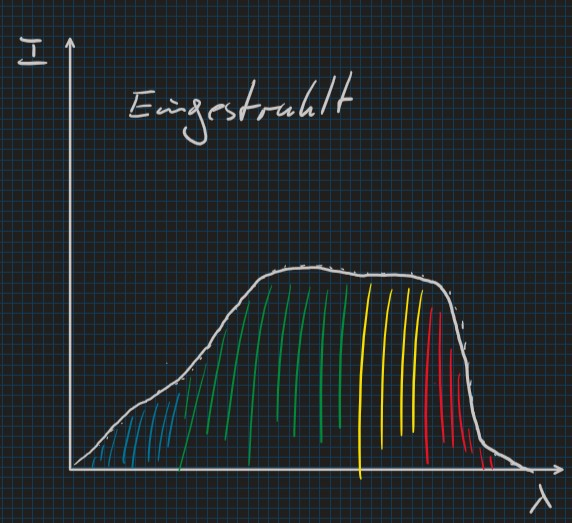
\includegraphics[width=0.4\linewidth]{entries/6/eingestrahlt_bb.jpg}}
    \qquad
    \subfloat[Intensitätsverteilung emittierter Wellenlängen des schwarzen Körpers.]{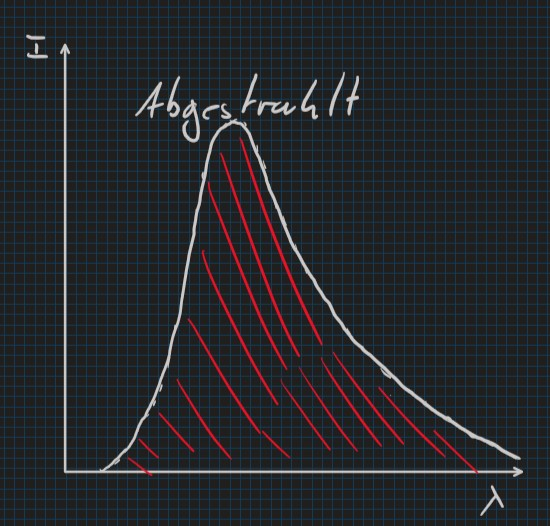
\includegraphics[width=0.4\linewidth]{entries/6/abgestrahlt_bb.jpg}}
    \caption{Schematische Darstellung absorbierter und emittierter Leistungen eines realen und eines schwarzen Körpers bei Bestrahlung durch einen willkürlich gewählten polychromatischen Strahler.}
    \label{fig:eingestrahlt}
\end{figure}

Die abgestrahlte maximale Wellenlänge ist hierbei eine Funktion ausschließlich der Temperatur des Materials gemäß des
Wien'schem Verschiebungsgesetzes
\begin{equation}
    \lambda_{max}=\frac{\SI{2897,8}{\mu mK}}{T}
\end{equation}
Das Vermögen eines Körpers Strahlungsleistung zu absorbieren sowie sie zu emittieren wird immer im Vergleich zum
schwarzen Strahler betrachtet und als einheitenloser Koeffizient zwischen 0 und 1 angegeben.
\begin{equation}
    \varepsilon = \frac{M_e}{M_{e,s}}
\end{equation}
\begin{equation}
    \alpha = \frac{M_a}{M_{a,s}}
\end{equation}
Nach Kirchhoff gilt hierbei \(\varepsilon = \alpha\).
Ein Körper ist immer bestrebt mit der Umgebung im thermodynamischen Gleichgewicht zu sein. Würde die abgestrahlte Leistung
nicht der eingestrahlten entsprechen würde der betrachtete Körper die absorbierte Leistung entweder aufintegrieren und
wohl irgendwann explodieren da seine innere Energie ins unermessliche anwüchse (Fall \(\varepsilon < \alpha\)) oder
die Bestrahlung des Körpers würde ihn de facto aktiv kühlen da er mehr Leistung abstrahlt als er zu absorbieren imstande
ist (Fall \(\varepsilon > \alpha\)).

Gibt es denn in der Natur schwarze Strahler? Ja, ich denke schon. Die (jede) Sonne. Was auch immer ich auf die Sonne
strahle wird weder reflektiert noch transmittiert sondern vollständig absorbiert.